% ------------------------------------------------------------------------------
% ------------------------------------------------------------------------------
% Relatório de Trabalho 2 de Algoritmos Numéricos 2
% André Barreto
% Igor Ventorim
% ------------------------------------------------------------------------------
% ------------------------------------------------------------------------------

\documentclass[
	11pt,				% tamanho da fonte
	oneside,			% para impressão apenas no verso. Oposto a twoside
	a4paper,			% tamanho do papel. 
	english,			% idioma adicional para hifenização
	brazil,				% o último idioma é o principal do documento
	]{article}


% ---
% PACOTES
% ---
\usepackage{lmodern}
\usepackage[T1]{fontenc}
\usepackage[utf8]{inputenc}
%\usepackage{indentfirst}
\usepackage{nomencl}
\usepackage{color}
\usepackage{graphicx}
\usepackage{microtype}
\usepackage{makeidx}
\usepackage{multirow,tabularx}
\usepackage{multicol}
\usepackage{float}
\usepackage{listings}
\usepackage{color}
\usepackage{hyperref}
\usepackage{cite}
\usepackage{url}
\usepackage[brazilian]{babel}
\usepackage[brazilian,hyperpageref]{backref}
\usepackage{amsmath}
\usepackage{mathtools,amssymb}
\usepackage{pgfplots}
\usepackage{lipsum}
\usepackage[portuguese,linesnumbered,vlined]{algorithm2e}	% Gerar pseudo-códigos
% ---

\chardef\_=`_
\newcommand{\specialcell}[2][c]{%
  \begin{tabular}[#1]{@{}c@{}}#2\end{tabular}}
  
% ---
% Configurações do pacote listings
% ---
\definecolor{mygreen}{rgb}{0,0.6,0}
\definecolor{mygray}{rgb}{0.571428571,0.571428571,0.571428571}
\definecolor{mymauve}{rgb}{0.5714285718,0,0.82}
\definecolor{codegreen}{rgb}{0,0.6,0}
\definecolor{codegray}{rgb}{0.571428571,0.571428571,0.571428571}
\definecolor{codepurple}{rgb}{0.5714285718,0,0.82}
\definecolor{backcolour}{rgb}{0.95,0.95,0.92}
\lstset{
	backgroundcolor=\color{white},
	basicstyle=\footnotesize,
	breakatwhitespace=false,
	breaklines=true,
	captionpos=b,
	commentstyle=\color{mygreen},
	deletekeywords={...},
	escapeinside={\%*}{*)},
	extendedchars=true,
	keepspaces=true,
	keywordstyle=\color{blue},
	language=C,
	otherkeywords={*,...},
	numbers=left,
	numbersep=5pt,
	numberstyle=\tiny\color{mygray},
	rulecolor=\color{black},
	showspaces=false,
	showstringspaces=false,
	showtabs=false,
	stepnumber=1,
	stringstyle=\color{mymauve},
	tabsize=2,
	title=\lstname
}
% ---
	
% ---
% Informações de dados para CAPA
% ---
\title{\textbf{Estudo Sobre a Influência do Reordenamento e Precondicionamento aplicados a Sistemas Esparsos de Grande Porte Utilizando Métodos Iterativos Não Estacionários}}
\author{
André Barreto e Igor Ventorim\\\\
\normalsize Universidade Federal do Espírito Santo\\
}
\date{2016}
% ---

% ---
% Configurações de aparência do PDF final
% ---
\definecolor{blue}{RGB}{41,5,195}

% informações do PDF
\makeatletter
\hypersetup{
	pdftitle={\@title}, 
	pdfauthor={\@author},
	pdfsubject={Escalonamento de Jobs},
	pdfcreator={LaTeX with abnTeX2},
	pdfkeywords={abnt}{latex}{abntex}{abntex2}{atigo científico}, 
	colorlinks=true,
	linkcolor=blue,
	citecolor=blue,
	filecolor=magenta,
	urlcolor=blue,
	bookmarksdepth=4
}
\makeatother
% --- 

% ---
% Compila o indice
% ---
\makeindex
% ---

% --- 
% Espaçamentos entre linhas e parágrafos 
% --- 
\setlength{\parindent}{1cm}
\setlength{\parskip}{0.2cm}
% ---

% ----
% Início do documento
% ----
\begin{document}
% ---

% Seleciona o idioma do documento
\selectlanguage{brazil}

% Retira espaço extra obsoleto entre as frases.
\frenchspacing

% Caminho da pasta de imagens
\graphicspath{ {Imagens/} }

% ------------------------------------------------------------------------------
% Página de Título
% ------------------------------------------------------------------------------
\begin{titlepage}
	\centering
	{\scshape \large Universidade Federal do Espírito Santo\par}
	{\large Departamento de Informática\par}
	\vspace{1cm}
	{\large André Barreto\\Igor Ventorim\par}
	
	\vfill
	
	{\LARGE \bfseries Estudo Sobre a Influência do Reordenamento e Precondicionamento aplicados a Sistemas Esparsos de Grande Porte Utilizando Métodos Iterativos Não Estacionários\par}
	\vspace{1cm}
	{\large Trabalho 2 de Algoritmos Numéricos 2\par}

	\vfill

	{\large Vitória\par}
	{\large 2016\par}
\end{titlepage}
\addtocounter{page}{1}

% ------------------------------------------------------------------------------
% Introdução
% ------------------------------------------------------------------------------
\section{Introdução}
Frequentemente os processos de solução de problemas das mais diversas áreas do conhecimento recaem na necessidade de resolver sistemas lineares. Na maioria das vezes esses sistemas são esparsos e de grande porte. Nesse contexto, o uso de métodos diretos torna-se desaconselhável, por limitações de tempo e memória. Em detrimento, as abordagens iterativas tornam-se mais atraentes.

Neste trabalho, será estudado o GMRES, método iterativo não estacionário, que caracteriza-se por buscar uma aproximação da solução dos sistemas lineares a partir de um subespaço. Este método também é conhecido como livre de matriz.

Os métodos iterativos não estacionários, apesar de bem fundamentados teoricamente, podem sofrer convergência lenta para problemas que surgem de aplicações típicas. Para resolver tal questão, deve-se considerar o uso de bons precondicionadores, que melhoram o condicionamento de uma matriz, acelerando a convergência. Além disto, deve-se considerar o uso de processos de reordenamento, que são simples trocas de linhas, reduzindo o número de operações com ponto flutuante durante a montagem das matrizes precondicionadoras.

Em suma, este trabalho tem como objetivo realizar um estudo sobre a utilização de métodos iterativos não estacionários no contexto de matrizes esparsas de grande porte e verificar a influência do ordenamento e o precondicionamento aplicado a essas matrizes.

Neste contexto, realizar tal estudo requer experimentos práticos com resultados visuais. Para tanto, na seção \ref{sec:expnum} serão apresentados experimentos numéricos para tal análise. Antes desta, na seção \ref{sec:refteo}, encontram-se resumos dos métodos e técnicas abordados. E por fim, a seção \ref{sec:conc} são discutidos brevemente os resultados obtidos.

% ------------------------------------------------------------------------------
% Referencial Teórico
% ------------------------------------------------------------------------------
\section{Referencial Teórico} \label{sec:refteo}

\subsection{Sistemas lineares de grande porte}
Sistemas lineares de grande porte aparecem como resultado da modelagem de vários problemas nas engenharias. A busca de métodos para resolução destes sistemas é muito abordada pela Ciência da Computação. Neste trabalho, resolveremos sistemas lineares $Ax = b$ esparsos de grande porte.

\subsection{Técnica de Compactação de matriz CSR}
O método de armazenamento de matrizes esparsas Compressed Sparse Row(CSR) é um método de armazenamento de matrizes esparsas que utiliza três vetores para armazenar os valores não nulos da matriz assim denominados $valA$, $rowPtrA$ e $colIndA$. O vetor AA armazena os valores não nulos da matriz, o vetor IA armazena os índices identificando a posição no vetor AA onde se inicia uma nova linha da matriz e o vetor JA armazena os índices referentes às colunas em que os elementos não nulos estão posicionados na matriz.

\noindent Exemplo:

\begin{align*}
AA &= [1, 1, 4, 2, 4, 1, 2, 1, 8, 2, 4, 1, 3, 6, 2, 1] \\
JA &= [0, 1, 4, 1, 2, 4, 0, 1, 2, 3, 2, 3, 0, 1, 2, 4] \\
IA &= [0, 3, 6, 10, 13, 17]
\end{align*}

\begin{equation*}
A = 
\begin{bmatrix}
  1 & 1 & 0 & 0 & 4 \\
  0 & 2 & 4 & 0 & 1 \\
  2 & 1 & 8 & 2 & 0 \\
  0 & 0 & 4 & 1 & 0 \\
  3 & 6 & 2 & 0 & 1
\end{bmatrix}
\end{equation*}

Utilizaremos o método CSR uma vez que os sistemas propostos são esparsos. O armazenamento de forma otimizada ́é crucial na eficiência do método numérico.

\subsection{Precondicionamento}
O objetivo dos pré condicionadores é acelerar a convergência do métodos iterativos, de forma que dado um sistema $Ax = b$, podemos encontrar uma matriz $M$ tal que  $M^{-1} Ax = M^{-1}b$ onde M será o pré condicionador. Deve-se levar em conta que seja uma boa aproximação para A e seja fácil de implementar. Caso essas características não sejam satisfeitas, acaba se tornando inviável o uso de pré condicionadores.

Existem vários tipos de implementação de pré condicionadores. Neste trabalho foi utilizado o pré condicionador baseado da fatoração LU incompleta (ILU) tal que $M = ~L~U$ onde ~L e ~U são fatorações LU aproximadas de A. Para pré condicionadores baseados na fatoração incompleta (ILU) é necessário armazenamento extra para L e U, a operação do pré condicionador se dá na operação produto matriz-vetor do método iterativo.

Para aplicação dos pré condicionadores no trabalho foram criadas três funções principais a partir de que se tenha as Matrizes L e U.

Esta função é responsável por gerenciar as funções que realizam as operações necessárias para aplicação no método GMRES, resolvendo a matriz triangular superior e inferior.
\begin{lstlisting}[language=C, caption=Aplicação Pré Condicionamento LU]
void precondLU(MAT* L, MAT* U, double* vet_out, double* vet, int N)
{
    // Precondicionamento:
    // Ax = b ---> MAx = Mb
    // Mb' = b
    //
    // Resolver:
    // LUvet_out = vet

    double *q = createVector(N); // Vetor auxiliar

    // Lq = vet
    MATRIX_forward(L, q, vet);

    // Uvet_out = q
    MATRIX_backward(U, vet_out, q);

    free(q);
}
\end{lstlisting}

Função que resolve a matriz triangular superior armazenada com CSR.
\begin{lstlisting}[language=C, caption=Matrix Forward ]
// --------------------------------------------------
//  * Solve CSR matrix by successive substituions
//  *------------------------------------------------
void MATRIX_forward(MAT* L, double* x, double *b)
{
	int i, j, N;
	double soma = 0;

    N = L->n;
	x[0] = b[0]/L->D[0];
	for(i = 1; i < N; i++){
		soma = 0;
		for(j = L->IA[i]; j < L->IA[i+1];j++){
			soma += x[L->JA[j]]*L->AA[j];
		}
		x[i] = (b[i] - soma)/L->D[i];
	}
}
\end{lstlisting}

Função que resolve a matriz triangular inferior armazenada com CSR.
\begin{lstlisting}[language=C, caption=Matrix Backward]
// --------------------------------------------------
//  * Solve CSR matrix by retro substituions
// --------------------------------------------------
void MATRIX_backward(MAT* U, double* x, double *b)
{
	int i, j, N;
	double soma;

    N = U->n;
	x[N-1] = b[N-1]/U->D[N-1];
	for(i = N-2; i >=0; i--){
		soma = 0;
		for(j = U->IA[i]; j < U->IA[i+1];j++){
			soma += x[U->JA[j]]*U->AA[j];
		}
		x[i] = (b[i] - soma)/U->D[i];
	}
}
\end{lstlisting}

\subsection{Reordenamento}
O pré condicionamento de matrizes pode ocasionar em preenchimento, ou seja elementos nulos em $A$ se tornam não nulo em $M$. Uma solução é o uso de reordenamento para reduzir o preenchimento causado pelo pré condicionador baseado na fatoração ILU, reduzindo o preenchimento consequentemente reduziremos o tempo de computação. Após o uso do reordenamento e encontrada uma solução do sistema, é necessário reordenar novamente para que se encontre o vetor solução original.

Existem várias técnicas de reordenamento para a redução de \textit{fill-ins} (preenchimentos). A técnica proposta neste trabalho é a RCM, que apresenta uma boa qualidade de solução, baixo tempo de execução e fácil implementação. O RCM trabalha tentando aproximar os elementos não nulos da diagonal principal, o que resulta em uma redução de \textit{fill-ins}. Para saber quão próximo os elementos não nulos estão da diagonal principal foram estabelecidas duas métricas: a largura de banda e o envelope. A largura de banda pode ser definida como a maior distância entre o primeiro elemento não-nulo da linha $i$ até a diagonal principal. Já o envelope como a soma das distâncias entre o primeiro elemento não-nulo de cada linha $i$ até a diagonal principal.

\subsection{Métodos Iterativos Não Estacionários}
Os métodos iterativos não estacionários diferem dos métodos estacionários pois os operadores matriciais que atuam sobre a aproximação da solução $x^{k-1}$ para produzir $x^k$ não são constantes ao longo do processo iterativo.

A matriz dos coeficientes $A$ e o vetor dos termos independentes $b$ não são alterados durante o processo iterativo e dependem de critérios de convergência relacionados a matriz dos coeficientes $A$, sendo seu objetivo transformar o sistema $Ax = b$ em um problema de minimização do resíduo $||r_k|| = min ||b - Ax_k||$.

\subsubsection{GMRES}
O GMRES (Generalized Minimal Residual) foi proposto por Saad e Schultz, em 1986. Ele se diferencia do método dos gradientes conjugados por não ser restrito a matrizes simétricas definidas positivas. Porém, com isso temos que o uso dos polinômios residuais torna mais difícil, assim como não temos garantia da aplicação do teorema espectral. Tem como objetivo minimizar a norma do resíduo do sistema $x = min ||b-Ax_k||$. Considerando $x_0$ solução inicial, uma aproximada $x_k$ é dada por $x_k = x_0 + z$  onde $z$ é um vetor do espaço de Krylov $K^k = span {(r0, Ar0,A^2r0,...,A^{k-1}r0)}$

\begin{equation*}
min(x \in x_0 + K^k) (||b-Ax||)_2
\end{equation*}

Cada iteração do método GMRES é muito cara. Para torná-lo viável computacionalmente é adotado o processo de reinicializar a formação dos vetores da base a cada k iterações.

\noindent Supondo $k=10$

\begin{align*}
\noindent Dados &: A,b,x_0 \\
V &= [u_1, u_2,...,u_10] \\
y &= (y_1, y_2, y_10) \\
x_{10} &= x_0 + \sum\limits_{j=1}^{10}y_j u_j
\end{align*}

O Algoritmo com esta modificação é chamado de GMRES com Restart, o qual foi utilizado para a realização do trabalho.\\

\begin{algorithm}[H]
	\Entrada{$A, b,lmax,x=0,k n$}
	\Saida{$x$}
	\Inicio {
		$\epsilon = tol (||b||)_2$\;
		$l=1$\;
		\Repeat{$ p < \epsilon$ e $ l >= lmax$}{
		  $i = 1, u_i = b - Ax, e_i = ||u_i||, u_i = u_i/e_i, p = e_i$\;
		  \While{$p > \epsilon$ e $i < k$}{
		      $u_{i+1} = Au_i$\;
		      \For{$j \longleftarrow 1$ \KwTo $i$}{
			      $h_{ji}$ = $u_{i+1}^t u_j$\;
			      $u_{i+1} = u_{i+1} - h_{ji} u_j$\;
			      
		      }
		      $h_{i+1,i} = (||u_{i+1}||)_2$\;
		      $u_{i+1} = u_{i+1}/h_{i+1,i}$\;
		      
		      \For{$j \longleftarrow 1$ \KwTo $i-1$}{
		      $h_{ji} = c_j h_{ji} + s_j h_{j+1,i}$\;
		      $h_{j+1,i} = -s_j h_{ji} + c_j h_{j+1,i}$\;
		      }
		      $ r = \sqrt{h_{ii}^2 + h_{i+1,i}^2} $\;
		      $ c_i = h_{ii}/r$\;
		      $ s_i = h_{i+1,i}/r$\;
		      $ h_{ii} = r (h_{i+1,i} = 0)$\;
		      $ e_{i+1} = -s_i e_i $\;
		      $ e_i = c_i e_i$\;
		      $ p = |e_{i+1}|$\;
		      $ i  = i+1$\;
		  }
		  $ i = i - 1$\;
		  \For{$j \longleftarrow i$ \KwTo $1$}{
		    $y_j = (e_j - \sum\limits{l=j+1}^{i} h_{jl} y_l )/h_{jj}$\;
		  }
		  $x = \sum\limits{j=1}^{i} y_j u_j$\;
		  $l = l + 1$\;		
	}
	}
	\caption{GMRES c/Restart}
\end{algorithm}

Como as matrizes que estão sendo trabalhadas tem tratamentos bem particulares e foram armazenadas com a técnica de compactação de matriz CSR, é necessário que tenham funções específicas para realizar algumas operações. Uma operação de grande relevância no método GMRES é a operação produto matriz vetor que pode ser vista nas linhas 5 e 7 do algoritmo.

Segue a baixo a implementação do algoritmo produto matriz vetor em linguagem C para uma matriz armazenada com o método CSR:

\begin{lstlisting}[language=C, caption=Produto Matriz Vetor (CSR)]
//----------------------------------------------------------------------------
 // Compute CSR matrix vector product
 //--------------------------------------------------------------------------
void MATRIX_matvec(MAT *A, double* x, double *b)
{
	int i,j;

	for( i = 0; i < A->n; i++)
	{
		for(j = A->IA[i]; j < A->IA[i+1];j++)
		{
			x[i] += A->AA[j] * b[A->JA[j]];
		}
	}
}
\end{lstlisting}

\textbf{Observação:} para alterar a tolerância do GMRES, o número máximo de ciclos e o parâmetro do pré-condicionador ILU, deve-se alterar o código do arquivo \textit{trab2.c}, nas linhas indicadas a seguir:

\begin{lstlisting}[language=C, caption=Definições de constantes]
#define P    0         // Parametro de ILU(P)
#define TOL  0.000001  // Tolerancia do GMRES
#define LMAX 1000      // Num. maximo de ciclos do GMRES
\end{lstlisting}

% ------------------------------------------------------------------------------
% Experimentos Numéricos
% ------------------------------------------------------------------------------
\section{Experimentos Numéricos} \label{sec:expnum}
Nesta seção será feito um estudo do método GMRES, com e sem precondicionamento e com e sem ordenamento RCM, ao avaliar os tempos e números de iterações consumidos ao resolver sistemas lineares esparsos de grande porte. Para tanto, serão apresentados 8 tabelas e 4 gráficos resultantes dos experimentos para realizar o comparativo.

\subsection{Hardware utilizado}
Os testes nesta seção foram executados em uma máquina com as seguintes configurações:

Ubuntu 16.04 64-bit \\
\indent Intel Core i7-3770 CPU @ 3.40GHz x 4 \\
\indent 8GB de memória

\subsection{Matrizes utilizadas}
Na tabela \ref{tab:matrizes} estão descritas as matrizes esparsas utilizadas nos experimentos desta seção.

\begin{table}[H]
\centering
\begin{tabular}{|l|l|l|l|}
\hline
\multicolumn{1}{|c|}{\textbf{Matriz}} & \multicolumn{1}{c|}{\textbf{Área de Aplicação}} & \multicolumn{1}{c|}{\textbf{n}} & \multicolumn{1}{c|}{\textbf{nnz}} \\
\hline
rail\_5177 & Transferência de Calor & 5177 & 35185 \\
\hline
aft01 & Problema de Acústica & 8205 & 125567 \\
\hline
FEM\_3D\_thermal1 & Problema Térmico & 17880 & 430740 \\
\hline
Dubcova2 & Problema 2D/3D & 65025 & 1030225 \\
\hline
\end{tabular}
\caption{Matrizes utilizadas nos experimentos}
\label{tab:matrizes}
\end{table}

\subsection{Experimentos}
Para cada uma das matrizes apresentadas na tabela \ref{tab:matrizes}, foi resolvido o sistema linear utilizando o método GMRES com e sem precondicionamento ILU(p), e com e sem ordenamento RCM. Serão apresentadas a seguir duas tabelas para cada matriz, relacionando o número na base de Krylov $k$, o parâmetro $p$ do método ILU, a quantidade de iterações e o tempo computacional gasto para encontrar a solução através do método GMRES, com as considerações sobre reordenamento e precondicionamento.

Para uma melhor compreensão do estudo da convergência, para cada matriz da tabela \ref{tab:matrizes} foram selecionados os valores de $k$ e $p$ que resultaram em um menor tempo de processamento utilizando o método GMRES. E com estes, foram elaborados gráficos do número de iterações em função do logaritmo do resíduo da solução ($iter \times log(||r||))$. Nos gráficos, as iterações vão na sequência $1, 10, 20, 30, ..., 100$.

Os testes foram executados com uma tolerância de $tol = 10^{-6}$. Este valor foi escolhido empiricamente pois o método converge em um tempo viável e a solução é suficientemente boa. Além disto, o numero máximo de iterações do GMRES é $max = 1000$. Quando um caso de teste não convergir e atingir o máximo, será indicado $max$ em ``Iterações'' e $\infty$ em ``Tempo''.

\subsubsection{rail\_5177} \label{sec:rail}
A matriz rail\_5177 é a de menor ordem ($n = 5177$), porém é a matriz que menos convergiu nos experimentos, de acordo com as tabelas \ref{tab:rail-sem-rcm} e \ref{tab:rail-com-rcm}. A solução do sistema só foi alcançada dentro do limite utilizando o GMRES com ILU(p).

O parâmetro do ILU(p) que melhor condicionou a matriz quando sem ordenamento RCM foi $p = 4$. E com o RCM, $p = 3$.

\begin{table}[H]
\centering
\begin{tabular}{l|l|l|l|l|l|l|}
\cline{2-7}
 &  \multicolumn{2}{ c| }{\textbf{GMRES}} & \multicolumn{2}{ c| }{\textbf{GMRES}} & \multicolumn{2}{ c| }{\textbf{GMRES}} \\
\multicolumn{1}{c|}{} & \multicolumn{2}{c|}{\textbf{(s/ Precond.)}} & \multicolumn{2}{c|}{\textbf{+ ILU(0)}} & \multicolumn{2}{c|}{\textbf{+ ILU($p>0$)}} \\
\hline 
\multicolumn{1}{|l|}{\textbf{k}} & \textbf{Iterações} & \textbf{Tempo} & \textbf{Iterações} & \textbf{Tempo} & \textbf{Iter.} & \textbf{Tempo} \\
\hline
\multicolumn{1}{|l|}{20}  & $max$ & $\infty$ & $max$ & $\infty$ & $max$ & $\infty$ \\
\hline
\multicolumn{1}{|l|}{50}  & $max$ & $\infty$ & $max$ & $\infty$ & 549   & 1.158005 \\
\hline
\multicolumn{1}{|l|}{100} & $max$ & $\infty$ & $max$ & $\infty$ & 68    & 0.171907 \\
\hline
\end{tabular}
\caption{Matriz rail\_5177 - Método GMRES sem ordenamento RCM}
\label{tab:rail-sem-rcm}
\end{table}

\begin{table}[H]
\centering
\begin{tabular}{l|l|l|l|l|l|l|}
\cline{2-7}
 &  \multicolumn{2}{ c| }{\textbf{GMRES}} & \multicolumn{2}{ c| }{\textbf{GMRES}} & \multicolumn{2}{ c| }{\textbf{GMRES}} \\
\multicolumn{1}{c|}{} & \multicolumn{2}{c|}{\textbf{(s/ Precond.)}} & \multicolumn{2}{c|}{\textbf{+ ILU(0)}} & \multicolumn{2}{c|}{\textbf{+ ILU($p>0$)}} \\
\hline 
\multicolumn{1}{|l|}{\textbf{k}} & \textbf{Iterações} & \textbf{Tempo} & \textbf{Iterações} & \textbf{Tempo} & \textbf{Iter.} & \textbf{Tempo} \\
\hline
\multicolumn{1}{|l|}{20}  & $max$ & $\infty$ & $max$ & $\infty$ & $max$ & $\infty$ \\
\hline
\multicolumn{1}{|l|}{50}  & $max$ & $\infty$ & $max$ & $\infty$ & 2600  & 3.934766 \\
\hline
\multicolumn{1}{|l|}{100} & $max$ & $\infty$ & $max$ & $\infty$ & 76    & 0.182442 \\
\hline
\end{tabular}
\caption{Matriz rail\_5177 - Método GMRES com ordenamento RCM}
\label{tab:rail-com-rcm}
\end{table}

\begin{figure}[H]
    \centering
    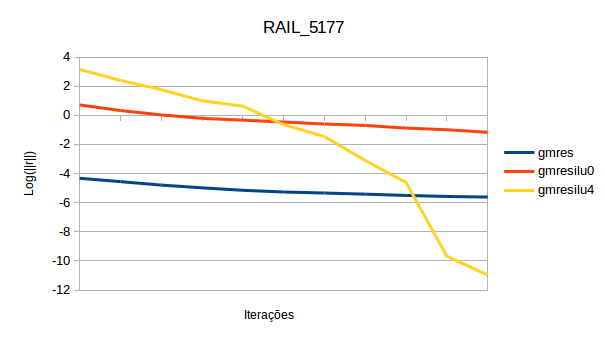
\includegraphics[width=\textwidth]{RAIL}
    \caption{Matriz rail\_5177 - Estudo da convergência do método GMRES}
    \label{fig:rail}
\end{figure}

\subsubsection{aft01} \label{sec:aft01}
aft01 é uma matriz oriunda de problemas de acústica, de ordem $n = 8205$ e $nnz = 125567$ valores não nulos. Esta matriz também se mostrou um tanto complexa, assim como a rail\_5177, com poucos casos de convergência. O diferencial desta matriz é que o GMRES sem precondicionamento gera resultados incorretos, convergindo rapidamente mas apresentando uma solução errônea. Nestes casos, foi marcado $erro$ nas tabelas \ref{tab:aft01-sem-rcm} e \ref{tab:aft01-com-rcm}.

O melhor valor de $p$ do ILU encontrado, tanto com e sem ordenamento RCM, foi tal que $p = 10$.

\begin{table}[H]
\centering
\begin{tabular}{l|l|l|l|l|l|l|}
\cline{2-7}
 &  \multicolumn{2}{ c| }{\textbf{GMRES}} & \multicolumn{2}{ c| }{\textbf{GMRES}} & \multicolumn{2}{ c| }{\textbf{GMRES}} \\
\multicolumn{1}{c|}{} & \multicolumn{2}{c|}{\textbf{(s/ Precond.)}} & \multicolumn{2}{c|}{\textbf{+ ILU(0)}} & \multicolumn{2}{c|}{\textbf{+ ILU($p>0$)}} \\
\hline 
\multicolumn{1}{|l|}{\textbf{k}} & \textbf{Iterações} & \textbf{Tempo} & \textbf{Iterações} & \textbf{Tempo} & \textbf{Iter.} & \textbf{Tempo} \\
\hline
\multicolumn{1}{|l|}{20}  & $erro$ & $-$ & $max$ & $\infty$ & 12 & 0.054555 \\
\hline
\multicolumn{1}{|l|}{50}  & $erro$ & $-$ & $max$ & $\infty$ & 12 & 0.054520 \\
\hline
\multicolumn{1}{|l|}{100} & $erro$ & $-$ & 85    & 0.313931 & 12 & 0.054545 \\
\hline
\end{tabular}
\caption{Matriz aft01 - Método GMRES sem ordenamento RCM}
\label{tab:aft01-sem-rcm}
\end{table}

\begin{table}[H]
\centering
\begin{tabular}{l|l|l|l|l|l|l|}
\cline{2-7}
 &  \multicolumn{2}{ c| }{\textbf{GMRES}} & \multicolumn{2}{ c| }{\textbf{GMRES}} & \multicolumn{2}{ c| }{\textbf{GMRES}} \\
\multicolumn{1}{c|}{} & \multicolumn{2}{c|}{\textbf{(s/ Precond.)}} & \multicolumn{2}{c|}{\textbf{+ ILU(0)}} & \multicolumn{2}{c|}{\textbf{+ ILU($p>0$)}} \\
\hline 
\multicolumn{1}{|l|}{\textbf{k}} & \textbf{Iterações} & \textbf{Tempo} & \textbf{Iterações} & \textbf{Tempo} & \textbf{Iter.} & \textbf{Tempo} \\
\hline
\multicolumn{1}{|l|}{20}  & $erro$ & $-$ & $max$ & $\infty$ & 13 & 0.051558 \\
\hline
\multicolumn{1}{|l|}{50}  & $erro$ & $-$ & $max$ & $\infty$ & 13 & 0.050558 \\
\hline
\multicolumn{1}{|l|}{100} & $erro$ & $-$ & 92    & 0.338417 & 13 & 0.050448 \\
\hline
\end{tabular}
\caption{Matriz aft01 - Método GMRES com ordenamento RCM}
\label{tab:aft01-com-rcm}
\end{table}

\begin{figure}[H]
    \centering
    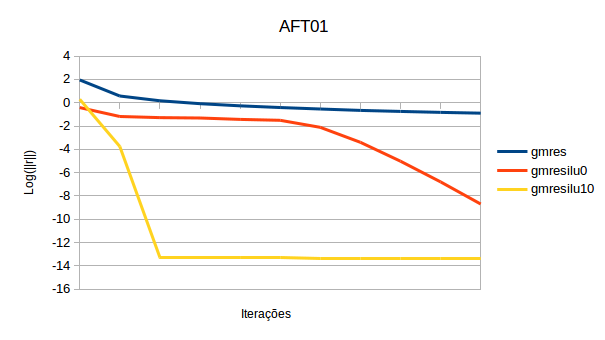
\includegraphics[width=\textwidth]{AFT01}
    \caption{Matriz aft01 - Estudo da convergência do método GMRES}
    \label{fig:aft}
\end{figure}

\subsubsection{FEM\_3D\_thermal1} \label{sec:fem}
A matriz FEM\_3D\_thermail1,  de ordem $n = 17880$ e $nnz = 430740$ mostrou-se uma matriz de fácil resolução, apesar de ordem elevada. Esta não foi capaz de convergir apenas quando utilizando GMRES sem precondicionamento e $k < 100$, de acordo com as tabelas \ref{tab:fem-sem-rcm} e \ref{tab:fem-com-rcm}.

Melhor valor para ILU(p): $p = 1$

\begin{table}[H]
\centering
\begin{tabular}{l|l|l|l|l|l|l|}
\cline{2-7}
 &  \multicolumn{2}{ c| }{\textbf{GMRES}} & \multicolumn{2}{ c| }{\textbf{GMRES}} & \multicolumn{2}{ c| }{\textbf{GMRES}} \\
\multicolumn{1}{c|}{} & \multicolumn{2}{c|}{\textbf{(s/ Precond.)}} & \multicolumn{2}{c|}{\textbf{+ ILU(0)}} & \multicolumn{2}{c|}{\textbf{+ ILU($p>0$)}} \\
\hline 
\multicolumn{1}{|l|}{\textbf{k}} & \textbf{Iterações} & \textbf{Tempo} & \textbf{Iterações} & \textbf{Tempo} & \textbf{Iter.} & \textbf{Tempo} \\
\hline
\multicolumn{1}{|l|}{20}  & $max$ & $\infty$ & 7 & 0.039565 & 5 & 0.056208 \\
\hline
\multicolumn{1}{|l|}{50}  & $max$ & $\infty$ & 7 & 0.043184 & 5 & 0.042400 \\
\hline
\multicolumn{1}{|l|}{100} & 188 & 1.446595   & 7 & 0.039589 & 5 & 0.046340 \\
\hline
\end{tabular}
\caption{Matriz FEM\_3D\_thermal1 - Método GMRES sem ordenamento RCM}
\label{tab:fem-sem-rcm}
\end{table}

\begin{table}[H]
\centering
\begin{tabular}{l|l|l|l|l|l|l|}
\cline{2-7}
 &  \multicolumn{2}{ c| }{\textbf{GMRES}} & \multicolumn{2}{ c| }{\textbf{GMRES}} & \multicolumn{2}{ c| }{\textbf{GMRES}} \\
\multicolumn{1}{c|}{} & \multicolumn{2}{c|}{\textbf{(s/ Precond.)}} & \multicolumn{2}{c|}{\textbf{+ ILU(0)}} & \multicolumn{2}{c|}{\textbf{+ ILU($p>0$)}} \\
\hline 
\multicolumn{1}{|l|}{\textbf{k}} & \textbf{Iterações} & \textbf{Tempo} & \textbf{Iterações} & \textbf{Tempo} & \textbf{Iter.} & \textbf{Tempo} \\
\hline
\multicolumn{1}{|l|}{20}  & $max$ & $\infty$ & 9 & 0.047200 & 6 & 0.050042 \\
\hline
\multicolumn{1}{|l|}{50}  & $max$ & $\infty$ & 9 & 0.046716 & 6 & 0.050021 \\
\hline
\multicolumn{1}{|l|}{100} & 188 & 1.394231   & 9 & 0.048806 & 6 & 0.050120 \\
\hline
\end{tabular}
\caption{Matriz FEM\_3D\_thermal1 - Método GMRES com ordenamento RCM}
\label{tab:fem-com-rcm}
\end{table}

\begin{figure}[H]
    \centering
    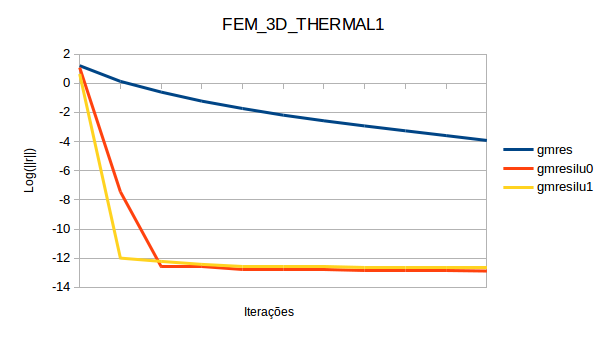
\includegraphics[width=\textwidth]{FEM}
    \caption{Matriz FEM\_3D\_thermal1 - Estudo da convergência do método GMRES}
    \label{fig:fem}
\end{figure}

\subsubsection{Dubcova2} \label{sec:dub}
Dubcova2 é a maior matriz utilizada nestes experimentos, com ordem $n = 65025$ e $nnz = 1030225$ valores não nulos. E ainda assim, esta converge mais facilmente que as menores matrizes estudadas até então. Veja nas tabelas \ref{tab:dub-sem-rcm} e \ref{tab:dubcova2-com-rcm} os testes realizados nesta matriz.

Para o precondicionamento ILU(p), foram econtrados $p = 1$ como o melhor caso não seja realizado o ordenamento RCM e $p = 5$ caso contrário.

\begin{table}[H]
\centering
\begin{tabular}{l|l|l|l|l|l|l|}
\cline{2-7}
 &  \multicolumn{2}{ c| }{\textbf{GMRES}} & \multicolumn{2}{ c| }{\textbf{GMRES}} & \multicolumn{2}{ c| }{\textbf{GMRES}} \\
\multicolumn{1}{c|}{} & \multicolumn{2}{c|}{\textbf{(s/ Precond.)}} & \multicolumn{2}{c|}{\textbf{+ ILU(0)}} & \multicolumn{2}{c|}{\textbf{+ ILU($p>0$)}} \\
\hline 
\multicolumn{1}{|l|}{\textbf{k}} & \textbf{Iterações} & \textbf{Tempo} & \textbf{Iterações} & \textbf{Tempo} & \textbf{Iter.} & \textbf{Tempo} \\
\hline
\multicolumn{1}{|l|}{20}  & $max$ & $\infty$  & $max$ & $\infty$ & 880 & 22.371890 \\
\hline
\multicolumn{1}{|l|}{50}  & 999   & 15.694150 & 141   & 2.765995 & 37  & 1.005747 \\
\hline
\multicolumn{1}{|l|}{100} & 252   & 5.957986  & 74    & 1.845755 & 37  & 1.015742 \\
\hline
\end{tabular}
\caption{Matriz Dubcova2 - Método GMRES sem ordenamento RCM}
\label{tab:dub-sem-rcm}
\end{table}

\begin{table}[H]
\centering
\begin{tabular}{l|l|l|l|l|l|l|}
\cline{2-7}
 &  \multicolumn{2}{ c| }{\textbf{GMRES}} & \multicolumn{2}{ c| }{\textbf{GMRES}} & \multicolumn{2}{ c| }{\textbf{GMRES}} \\
\multicolumn{1}{c|}{} & \multicolumn{2}{c|}{\textbf{(s/ Precond.)}} & \multicolumn{2}{c|}{\textbf{+ ILU(0)}} & \multicolumn{2}{c|}{\textbf{+ ILU($p>0$)}} \\
\hline 
\multicolumn{1}{|l|}{\textbf{k}} & \textbf{Iterações} & \textbf{Tempo} & \textbf{Iterações} & \textbf{Tempo} & \textbf{Iter.} & \textbf{Tempo} \\
\hline
\multicolumn{1}{|l|}{20}  & $max$ & $\infty$  & 198 & 2.913908 & 15 & 0.356196 \\
\hline
\multicolumn{1}{|l|}{50}  & 999   & 16.022811 & 49  & 1.027727 & 15 & 0.360827 \\
\hline
\multicolumn{1}{|l|}{100} & 252   & 6.092857  & 49  & 0.995358 & 15 & 0.363706 \\
\hline
\end{tabular}
\caption{Matriz Dubcova2 - Método GMRES com ordenamento RCM}
\label{tab:dubcova2-com-rcm}
\end{table}

\begin{figure}[H]
    \centering
    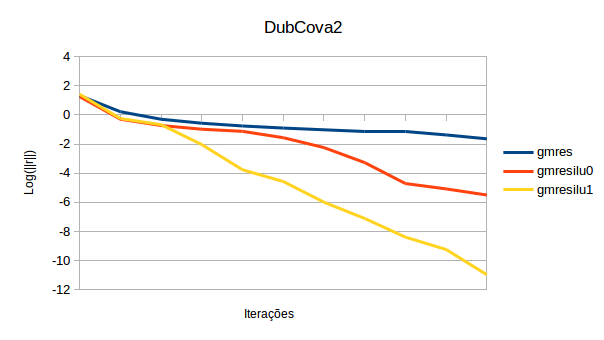
\includegraphics[width=\textwidth]{DubCova}
    \caption{Matriz Dubcova2 - Estudo da convergência do método GMRES}
    \label{fig:dub}
\end{figure}

% ------------------------------------------------------------------------------
% Conclusão
% ------------------------------------------------------------------------------
\section{Conclusão} \label{sec:conc}
Da série de experimentos realizados na seção \ref{sec:expnum}, podemos avaliar o método não estacionário GMRES e o uso de reordenamento e precondicionadores no mesmo.

É notável perceber que o GMRES possui bons resultados para sistemas esparsos de grande porte, uma vez que foi pensado para isto. Mas vemos que, simplesmente utilizado, o método pode sofrer de uma convergência lenta, tornando-se inviável, ou até mesmo produzir resultados incorretos. Este último pode ser observado nos testes da matriz aft01 (seção \ref{sec:aft01}). Quanto a velocidade de convergência, em todas as matrizes houve ao menos um caso em que o GMRES puro não obteve a solução no limite de iterações. Em destaque, para a matriz rail\_5177, que não convergiu para qualquer teste (seção \ref{sec:rail}).

Como esperado, o GMRES puro não garante, em muitos casos, bons resultados, principalmente em questão de tempo. Agora, quando adicionado a ele o uso do precondicionador ILU(p), observamos resultados muito melhores. Por exemplo, no experimento da matriz Dubcova2 (seção \ref{sec:dub}), na tabela \ref{tab:dub-sem-rcm}, e $ k = 50 $, ocorre um ganho muito grande de tempo e iterações. De 999 para 141 iterações e de aproximadamente 15 segundos para 3. Uma redução significante devido ao precondicionamento da matriz.

Ainda sobre o precondicionamento ILU(p), vemos que o parâmetro $ p $ é bastante relevante no método. Isto pode ser ilustrado nos testes da matriz rail\_5177 (tabelas \ref{tab:rail-sem-rcm} e \ref{tab:rail-com-rcm}), onde para $ p = 0 $, não houve ganho algum se comparado com o GMRES simples, pois ambos não convergiram. Em contrapartida, para $ p = 4 $, foi alcançado uma resposta em tempo extremamente viável. E se observados os outros experimentos, vemos que o melhor valor de $ p $ não é o maior nem possui um padrão entre os casos. O melhor valor depende da matriz proposta, sendo definido, portanto, empiricamente.

Quanto ao ordenamento RCM, podemos observar sua influência positiva claramente no experimento da matriz Dubcova2 (\ref{sec:dub}). Sem ordenamento, para $ k = 20 $, o método converge apenas quando aplicado ILU(1), e ainda converge lentamente, com 880 iterações em 22 segundos. Agora, quando aplicado o RCM, este tempo cai para 0.35 segundos em apenas 15 iterações, utilizando $ p = 5 $, o novo melhor parâmetro do ILU. Além disto, também passa a convergir para ILU(0), o que não era verdade quando sem o ordenamento. 

Mas o processo RCM nem sempre surte efeitos positivos, mantendo os tempos e iteração praticamente iguais. E em alguns poucos casos, aparentemente pode até piorar a convergência do GMRES. Assim como para o valor de $ p $, a efetividade do ordenamento RCM não é fácil de ser prevista. Logo, deve-se determinar o seu uso de acordo com a matriz a ser resolvida do sistema.

Com estas análises, vemos que resolver sistemas lineares esparsos de grande porte não é trivial. Devem ser considerados todos estes métodos - armazenamento, reordenamento e pré-condicionamento da matriz e o método de resolução do sistema - para que seja viável resolver muitos problemas que surgem de aplicações reais.

\end{document}